\documentclass[twocolumn]{article}%
\usepackage[utf8]{inputenc}
\usepackage[T1]{fontenc}
\usepackage{geometry}
\usepackage{cuted}
\usepackage{lipsum}
\title{Handwritten Equation Recognizer (HER)}
\author{William Jussiau, Johnson Loh, David Schmidt}
\date{\today}
\setlength\columnsep{3em}
\usepackage{graphicx}

\begin{document}


%\begin{strip}
%  \vspace*{\dimexpr-\baselineskip-\stripsep\relax}
%  \centering
%  \maketitle
%  \vskip\baselineskip
%%\noindent\makebox[\textwidth]{\rule{1.1\paperwidth}{0.4pt}}
%  \vskip\baselineskip
%\end{strip}

\twocolumn[
  \begin{@twocolumnfalse}
    \maketitle
    \begin{abstract}
     	    The Handwritten Equation Recognizer (HER) is an approach to apply machine learning techniques in the context of pattern recognition. The focus of this work is to identify handwritten equations based on image data. The identification procedure consists of two steps: cluster the pixels in the image to symbols and then classify the recognized clusters as mathematical symbols.
    \end{abstract}
  \end{@twocolumnfalse}
]

 

	
	\section{Introduction}
		The field of handwriting recognition is an interesting application task for advanced machine learning algorithms. In tournaments like the Competition on Recognition of Handwritten Mathematical Expressions (CROHME) \cite{crohme}, different teams compare their state of the art algorithms on a huge dataset. Usually, this dataset consists of stroke sequences, which describe the generation of a whole mathematical formula.\\
		In contrast to using this sort of data (i.e. stroke sequence), our approach is using the image of the mathematical expression. The information of how a symbol is actually constructed is not used. Instead, the image is preprocessed into a binary image using the an optimal threshold. Then, based upon the pixel occupancy and their location, two steps of machine learning are applied. The first step is a clustering algorithm that enables us to get the location and extent of each symbol in the formula. With this information, we can then apply the second step on each cluster of pixels: classification. Each symbol extracted by the clustering step is to be recognized as a known mathematical glyph using a classifier.  Hence, it is possible to reconstruct the handwritten formula.
		The main part of our work was done with MATLAB. However, a part of the classification process was done in Python with the library TensorFlow.
	    	    
	    
	\section{Proposed method}
	\subsection{Clustering}
		The first algorithm to be applied aims at splitting the mathematical formula into single symbols. The method used in this project for identifying the symbols is the hierarchical agglomerative clustering algorithm. Using the functions provided in the Statistics and Machine Learning Toolbox from Matlab \cite{sml_matlab} the implementation is straight forward. The whole image is converted into a data array containing the two-dimensional coordinates of the occupied pixels in the image. Then the cluster tree is built using the Euclidean distance and single linkage as the cluster distance. Based on the generated dendrogram, a specified number of clusters can be derived. The amount of clusters can either be manually specified by the user or it can be generated by a cutoff distance $d_{cutoff}$. In this case, it makes sense to define this cutoff threshold as:
		\begin{equation}
		d_{symbol} > d_{cutoff} > \sqrt{\Delta x^2 + \Delta y^2}
		\end{equation}
		$\Delta x$ and $\Delta y$ denote respectively the horizontal and vertical pixel spacing. $d_{symbol}$ denotes the space between symbols. To provide an output for the following processing steps the bounding box of each recognized symbol is returned.
		
	\begin{figure}[htp]
	\centering
	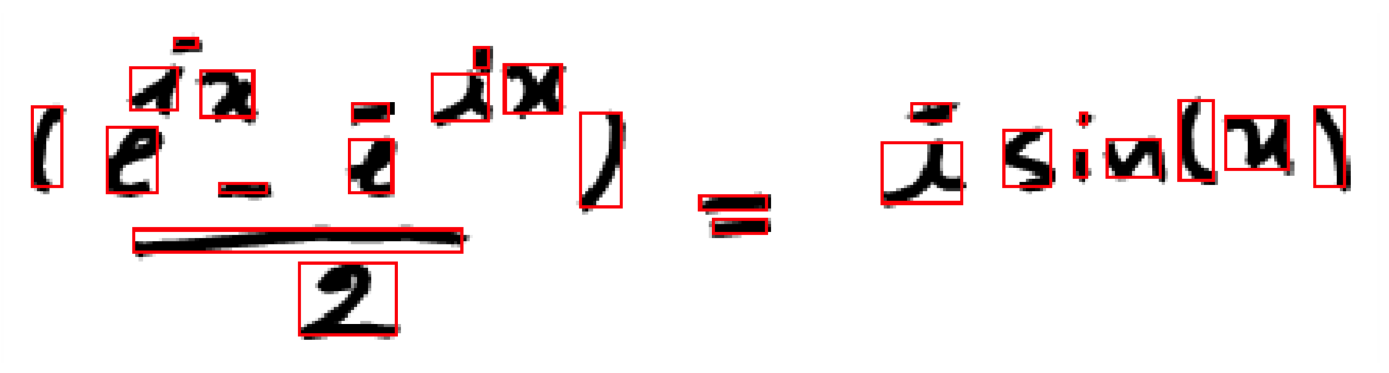
\includegraphics[scale=0.31]{images/cluster.png}
	\caption{Example - Clustering of a formula}
	\end{figure}
	
			The advantage of the hierarchical agglomerative clustering compared to other clustering methods is that it does not depend on the initialization of the clusters centres. As the assumption of the proposed method is that a symbol is defined as a connected space in the image space, the single linkage method is the most suited way to identify these symbols. The difficulties regarding symbols that are not connected in space (e.g. equal sign) can be solved by weighting vertical pixel space less than horizontal pixel space ($\Delta x > \Delta y$). 
		However, an obvious disadvantage is that connected symbols in some handwritings may be recognized as one single symbol. Another problem is to automatically define the number of symbols inside a given equation. Identifying the right point in the dendrogram is not trivial, as the horizontal pixel distance between the connection of two symbols and inside the symbol itself is the same.
	

	\subsection{Classification using traditional methods}
		As a second step, we want to recognize every single symbol extracted from the equation by the clustering algorithm. To do this, we will first access to a database regrouping a lot of single mathematical symbols as image files. Then, we will train several classifiers and compare their performance. Finally, we will be able to choose the best classifier to use for a working Handwritten Equation Recognizer.
		
	\paragraph{The dataset}
	The database we chose is called \texttt{HASYv2} \cite{hasyv2}, a publicly available, and free of charge dataset of
single symbols for computer vision applications. It contains a total of $168,233$ images of $369$ different classes. Symbols that lie in this dataset range from the Latin and Greek alphabets to numbers, with specific mathematical symbols on top of it (e.g. $\int, \supset, \sum, \coprod, ...$). Each entry of the dataset is a $[32\times32]$, black \& white, \texttt{png} image representing a particular symbol. A hundred examples of images taken from the dataset are displayed below.

	\begin{figure}[htp]
	\centering
	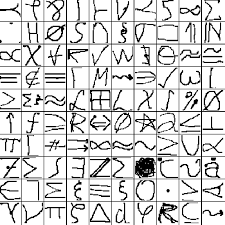
\includegraphics[scale=0.9]{images/hasyv2.png}
	\caption{An example of the HASYv2 dataset}
	\end{figure}


	There may be some counter-instinctive entries in the database, but it is known and intended. Especially:
	\begin{itemize}
	\item Two different symbols can have the same representation. For example, the symbols for a sum and the uppercase Greek \textit{sigma} are both represented by a $\Sigma$, but they have different meanings. This difference is relevant in the original field of application of this database, since the meaning of a symbol was paramount. The approach they used to recognize was different and more advanced, such that the meaning of the symbols were also taken into account before constructing the whole expression.
	\item Two different representations can correspond to the same symbol. For example,  $\varphi$ and $\phi$ are a same representation of the Greek letter \textit{phi}. This allows more modularity because a higher number of handwritings may be recognized.
	\end{itemize}
	We wanted to stick to the provided dataset as much as possible, so we kept all the entries that looked like duplicates as well as symbols that were rarely (to say the least) used in simple mathematical formulas. More details about the dataset can be found in the reference \cite{hasyv2} where several other aspects of the data are explored.
	
	\paragraph{Acquiring the data}
	As the dataset was quite large (especially in terms of number of files, which was an issue when trying to transfer or upload these files), we wanted to gather all the data in a single file. Every image was read with MATLAB, as a $[32\times32\times 3]$ vector (each pixel with its three RGB values). Then, it was reshaped into a single $[1\times1024]$ vector (unrolled, logical vector). Hence, the whole dataset consisted in a decent-sized $[168233 \times 1024]$ matrix which was stored in a \texttt{.mat} file. It allowed us to reduce the memory size of the database from several hundreds megabytes to $10.1$Mb. Additionnally, a simple \texttt{load} instruction would enable us to acquire all the data in a workspace.
	
	
	\paragraph{Different approaches to classification}
	The aim of this classification task is quite straightforward: we want to be able to automatically give the class of a given symbol among the 369 classes that exist. Considering the size of the data, we decided to use only MATLAB built-in classifiers rather than our own. The training time were decent with MATLAB functions and we assumed they would have been way higher with our, non-optimized or naive routines. Usually, we have used a training set accounting for 50 to 60\% of the data (the rest being test data).
	
	\subparagraph{What classifiers?}
	Without a priori knowing what kind of classifier would perform the best (in terms of training/prediction time and accuracy), we tried every classifier proposed by MATLAB. They all rely on classic algorithms, namely:
	\begin{itemize}
	\item k-nearest-neighbours
	\item Naïve Bayes
	\item Classification Tree
	\item Linear Discriminant Analysis
	\item Support Vector Machines
	\end{itemize}
	
	For the classifiers that we did not study during the unit, we mainly referred to MATLAB's documentation and online resources, where the algorithms are explained.
	
	\subparagraph{Dimensionality reduction}
	To try to compute a number of features that would be relevant to our problem, we wanted to compute the accuracy of each of our models with variable dimensionality, and then conclude on the number of dimensions we would take.
	We used dimensionality reduction in form of a Principal Component Analysis. We gradually decreased from $1024$ features to $2$ (each time halving the number of features), and evaluated the accuracy of each model. A summary plot is given below (with the number of features up to 128 only).
	
	\begin{figure}[htp]
	\centering
	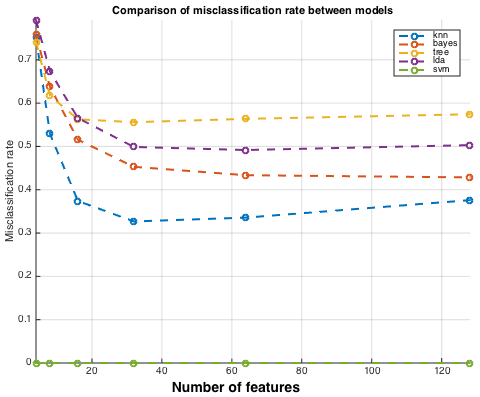
\includegraphics[scale=0.45]{images/error_vs_dimension.png}
	\caption{Models error versus dimensionality}
	\end{figure}
	
	Overall, the performance of the models increase with a higher number of features, and lies between $0.3$ and $0.6$ when the dimensionality is above $8$. However, it is almost constant from 64 features upwards, so we don't have any benefit in keeping a dimensionality that high. It is even noticeable that the k-nn classifier has a minimum classification rate for a number of features equal to 32. Hence, for the following, we will reduce the dimension of our data to 64 to have a good balance between all the models. Also, note that the SVM plot shows a misclassification rate of 0, because we were unable to run it (due to memory overload - it will be discussed in the following section).
	
	
	\subparagraph{A comparison between models}
	Knowing that we could use a Principal Component Analysis to reduce the number of features of an image from $1024$ to $64$ with satisfying performance, we wanted to assess the performance of the models we used. To have a good idea of the performance of the models (ensuring low error and predicting a result fast enough), we ran two analyses: estimate the accuracy of a model with respect to the number of classes considered (i.e. lower than 369), and estimate the prediction time taken by a trained model. It would then allow us to estimate beforehand the performance we could expect from the models, and compare reliably the models to a broader extent. It also allows us to predict the performance of a model with a similar dataset with a different number of symbols (or, if we wanted to add symbols to that dataset. Below are given the two plots produced by this analysis, with a number of classes considered from 12 to 92.
	
	\begin{figure}[h!]
	\centering
	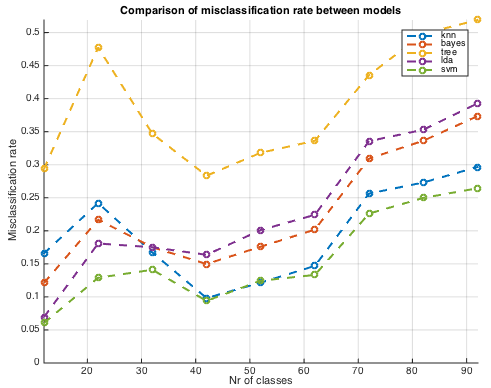
\includegraphics[scale=0.45]{images/error_vs_nclasses.png}
	\caption{Models error versus number of classes}
	\label{errorVSnClasses}
	\end{figure}
	
	Overall, as the dataset increases in complexity (i.e. more classes), the misclassification rate of every model increases. It may be interesting to notice that the models that perform well with 2 classes are not necessarily those that perform the best with a higher number of classes. With two classes, SVM and LDA show around 6\% of misclassification for 2 classes whereas k-nn shows 16\%. However, when 92 classes are considered, SVM shows 26\%, k-nn has 30\% and LDA has 39\%. Note that this plot should not necessarily taken as a reference, because the classes are added sequentially: the first two classes are $A$ and $B$, then comes $C$, etc. Thus, there may be variations due to the similarity or dissimilarity of adjacent classes in the dataset. 
	
	
	\begin{figure}[h!]
	\centering
	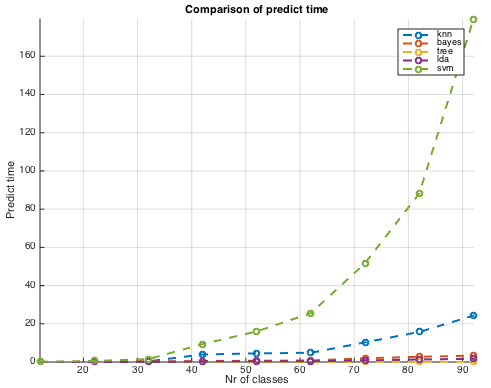
\includegraphics[scale=0.45]{images/time_vs_nclasses.png}
	\caption{Models predict time versus number of classes}
	\label{timeVSnClasses}
	\end{figure}
	
	Figure \ref{timeVSnClasses} illustrates one of the problems we encountered with this dataset: an enormous prediction time. The training time was also big to some extent, but once the model is saved there is no need for training anymore. The plot above shows that the models overall predict quite fast a solution on a test set, with both SVM and k-nn tending to have polynomial time complexity. Indeed, k-nn computes the distance between each points so its prediction time increases as a polynomial. The shape of the curve for the SVM can also be explained, knowing how MATLAB processes multi-class classification with SVM. It seems that there is no multi-class extension of the SVM more efficient than training binary SVM in a one-versus-one pattern. Hence, MATLAB actually trains $\frac{n(n-1)}{2}$ SVM, where $n$ is the number of classes in the dataset. For 369 classes, this would represent $67886$ binary models, that would take a tremendous time to train... and do not even fit in memory as a whole. This is the reason why we abandoned SVM - despite its really good accuracy -, because it was impossible to train with that many classes.
	
	\subparagraph{Partial conclusion}
	This analysis enabled us to spot several interesting characteristics of our models, and gave us hints on which one to use for our solution. A decent number of features seem to be 64, reached with standard PCA on the whole dataset. With all the classes considered, the SVM model computed by MATLAB is too large to fit in memory, thus we stop using it. We can rank the remaining models in terms of accuracy (the misclassification rate of the model is indicated between parentheses):
	\begin{enumerate}
	\item k-nn (32\%)
	\item Naïve Bayes (42\%)
	\item LDA (50\%)
	\item Classification Tree (58\%)
	\end{enumerate}
	
	
	\subsection{Classification using neural nets}	
	
	In recent years neural nets were very successfully applied to image recognition problems like the one presented above. Therefore we used the Matlab NeuralNet Toolbox to create and train a traditional neural net and the Keras package based on python and TensorFlow to apply the process for a convolutional neural network. The drawback of neural nets is their relatively large training time which makes it hard to evaluate them in a good manner. We mostly ran only one training process for each architecture.
	\subparagraph{Traditional neural net}
	Using Matlabs built-in NN Toolbox we trained NNs with a different amount of training data, input dimensions and hidden units in the one hidden layer we used. As more training data is always better we basically took as much as the run time of the training process allowed us to as it scaled linear with the amount of train data. We mostly used 30\% to 40\% of the whole set and the rest we splitted in half for test and validation. The input dimension also played a big role in the run time but using the results from the previous section we settled on values between 30 and 60. The number of hidden units were almost maxed out as we got close to filling up the complete RAM and Matlab actually did not allow us to go far beyond 500 hidden units. We experimented with values from 150 to 500 therefor. As the training processes took about 3 to 7 hours depending on the configuration we could not run a search over all the parameters so played with them using our intuition and understanding. The best neural network achieved a misclassification rate of only 31\% on the test set using only 36 input dimensions and 250 hidden units.
	\subparagraph{Convolutional NN}
	We tried to classify some examples of the data set ourselves to have a feeling for what error rate is actually achievable (at least by humans). We approximated the human error rate at about 20\% to 30\% so we were quite satisfied with the traditional NN. However as we applied the trained model on the symbols retrieved out of images by the clustering process we had to realize that the neural net could not generalize to different stroke widths and input data (as we had to resize and apply a binarizer the results seemed to be a bit artificial and not well represented by the training set we used). As Convolutional NNs tend to better generalize on image data \cite{lenet} we wanted to try them out using Keras \cite{keras} in python. With the filter sizes, the number of features, the number of convolutional layers, dropout regularization etc. we had an even larger space of parameters to tune, however the actual input dimension was not one of them as the way a CNN works does not require this step and it could not even handle PCA-reduced data very well. Surprisingly the training process was much faster giving often (for different sets of parameters) after an hour of training an error rate of below 30\% already. With this it would have been actually achievable to perform systematic parameter exploration if we had more time. The best performing CNN constructed and trained by us achieved a misclassification rate of only 21\% with 2 convolutional layers (using pooling) and 64 features in the last one, applying an additional traditional hidden layer of 512 units.
	% TODO write something about generalization to our data
	
	\section{Conclusion}
	
	\begin{thebibliography}{9}
		\bibitem{crohme} 
		International Conference on Frontiers in Handwriting Recognition in Shenzen, China (ICFHR),
		\\\texttt{http://ivc.univ-nantes.fr/CROHME/}
		
		\bibitem{sml_matlab} 
		Statistics and Machine Learning Toolbox, The MathWorks, Inc., 1994-2017,
		\\\texttt{https://au.mathworks.com/products/statistics.html}
		
		\bibitem{hasyv2}
		Thoma, M. (2017), The HASYv2 dataset
		
		\bibitem{lenet}
		LeNet-5, convolutional neural networks
		\\\texttt{http://yann.lecun.com/exdb/lenet/}
		
		\bibitem{keras}
		Keras: Deep Learning library for Theano and TensorFlow
		\\\texttt{https://keras.io}
		
		
	\end{thebibliography}

\end{document} 




















